\documentclass{standalone}
\usepackage{tikz}
\usetikzlibrary{automata,positioning}
\begin{document}
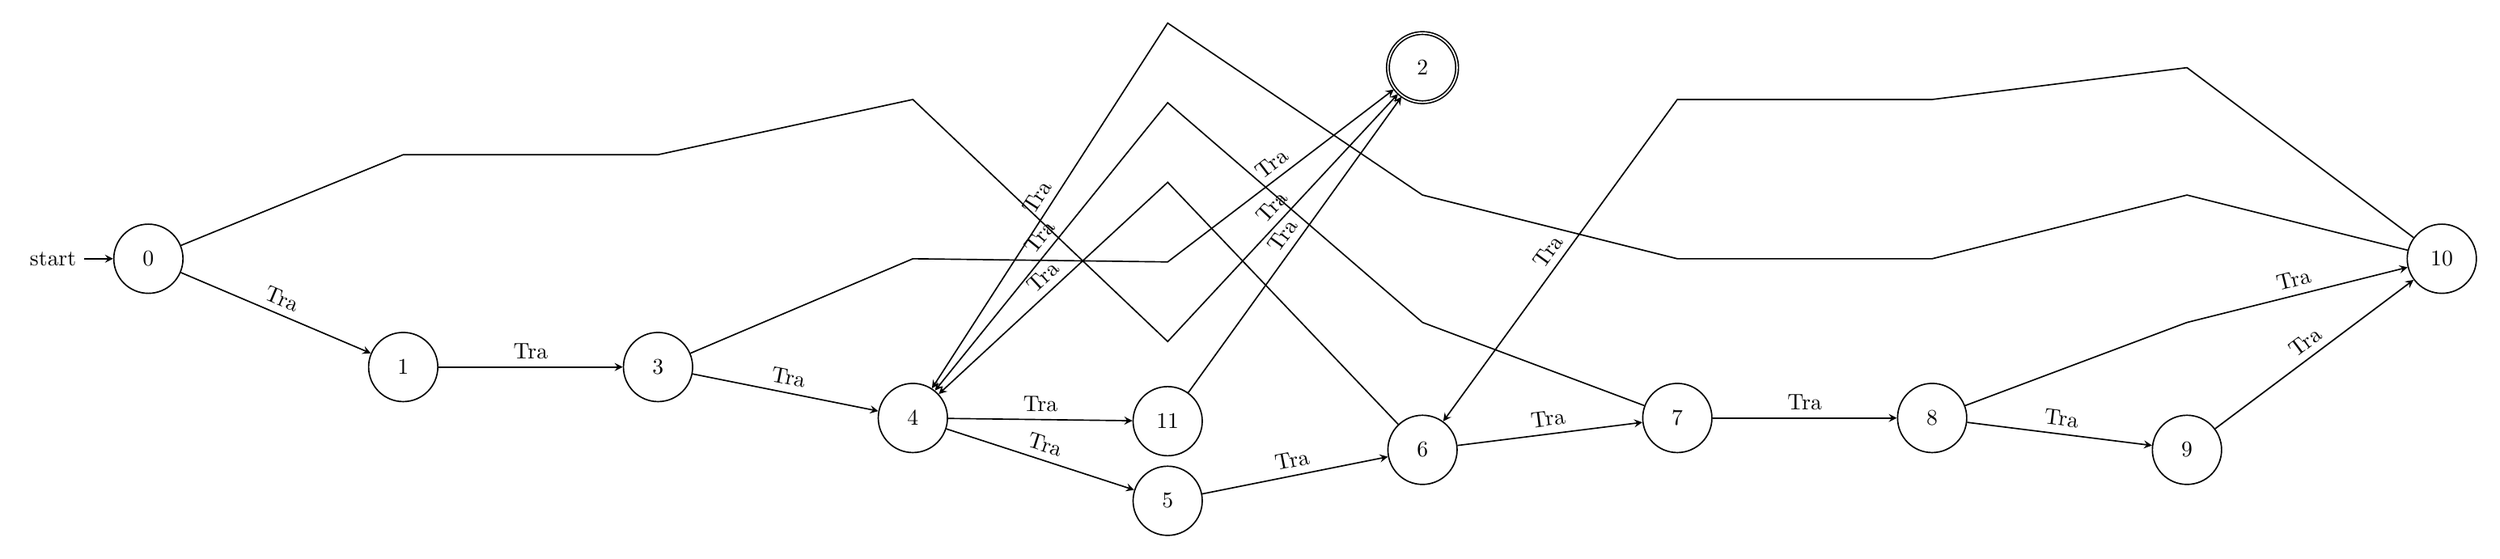
\begin{tikzpicture}[->,>=stealth,auto,node distance=2.5cm,semithick,every state/.style={minimum width=1cm, minimum height=1cm, text width=0.75cm,align=center}]
\node[state, initial] (0) at (0,5.0) {0};
\node[state] (1) at (4,3.3) {1};
\node[state, accepting] (2) at (20,8.0) {2};
\node[state] (3) at (8,3.3) {3};
\node[state] (4) at (12,2.5) {4};
\node[state] (5) at (16,1.2) {5};
\node[state] (6) at (20,2.0) {6};
\node[state] (7) at (24,2.5) {7};
\node[state] (8) at (28,2.5) {8};
\node[state] (9) at (32,2.0) {9};
\node[state] (10) at (36,5.0) {10};
\node[state] (11) at (16,2.45) {11};
\draw[->, rounded corners=0pt] (0) -- (4,6.633333333333333) -- (8,6.633333333333333) -- (12,7.5) -- (16,3.7) -- (2) node[midway, sloped, above] {Tra};
\draw[->, rounded corners=0pt] (3) -- (12,5.0) -- (16,4.95) -- (2) node[midway, sloped, above] {Tra};
\draw[->, rounded corners=0pt] (6) -- (16,6.2) -- (4) node[midway, sloped, above] {Tra};
\draw[->, rounded corners=0pt] (7) -- (20,4.0) -- (16,7.45) -- (4) node[midway, sloped, above] {Tra};
\draw[->, rounded corners=0pt] (8) -- (32,4.0) -- (10) node[midway, sloped, above] {Tra};
\draw[->, rounded corners=0pt] (10) -- (32,6.0) -- (28,5.0) -- (24,5.0) -- (20,6.0) -- (16,8.7) -- (4) node[midway, sloped, above] {Tra};
\draw[->, rounded corners=0pt] (10) -- (32,8.0) -- (28,7.5) -- (24,7.5) -- (6) node[midway, sloped, above] {Tra};
\path (0) edge node[midway, sloped, above] {Tra} (1);
\path (1) edge node[midway, sloped, above] {Tra} (3);
\path (3) edge node[midway, sloped, above] {Tra} (4);
\path (4) edge node[midway, sloped, above] {Tra} (5);
\path (5) edge node[midway, sloped, above] {Tra} (6);
\path (6) edge node[midway, sloped, above] {Tra} (7);
\path (7) edge node[midway, sloped, above] {Tra} (8);
\path (8) edge node[midway, sloped, above] {Tra} (9);
\path (9) edge node[midway, sloped, above] {Tra} (10);
\path (4) edge node[midway, sloped, above] {Tra} (11);
\path (11) edge node[midway, sloped, above] {Tra} (2);
\end{tikzpicture}
\end{document}